\chapter{固液界面}

\section{液体对固体的润湿}

主要有\{粘附,浸渍,铺展\}润湿。

\begin{enumerate}
    \item 粘附润湿 $W_a = \left(\gamma_{sg} + \gamma_{lg}\right) - \gamma_{s/l} \geq 0$
    \item 浸渍润湿 $W_i = \gamma_{sg} - \gamma_{sl} \geq 0$
    \item 铺展润湿 $S = S_{sg} - \left(\gamma_{sl} + \gamma_{lg}\right) \geq 0$
\end{enumerate}

\section{接触角方程}

\begin{figure}[h]
    \centering
    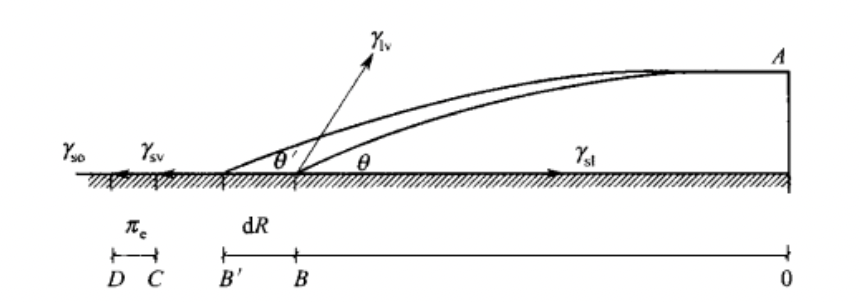
\includegraphics[width=0.8\textwidth]{images/sl_surface.png}
    \caption{液相与固相之间的接触角之间的关系}
\end{figure}

\begin{equation}
    \cos \theta = \frac{\gamma_{sg} - \gamma_{sl}}{\gamma_{lg}}
\end{equation}

\section{低能固体的表面特征量 $\gamma_c$}

Zisman 研究了各种液体在光滑低能表面上的接触角 $\theta$ 如何随液体的表面张力变化而变化。

\begin{equation}
    \cos \theta = b - c \gamma_{lv}
\end{equation}
